\section{Multiplicação por Escalar}

Dado um vetor $\overrightarrow{v} \neq \overrightarrow{0}$ e um número real
$\alpha \neq 0$, define-se o produto $\alpha \overrightarrow{v}$ como o vetor
que satisfaz (Figura~\ref{fig:fig1.19}):

\begin{itemize}
    \item \textbf{Módulo:} $|\alpha \overrightarrow{v}| = |\alpha|
      |\overrightarrow{v}|$;
    \item \textbf{Direção:} $\alpha \overrightarrow{v} \parallel
      \overrightarrow{v}$;
    \item \textbf{Sentido:} $\alpha \overrightarrow{v}$ tem o mesmo sentido de
      $\overrightarrow{v}$ se $\alpha > 0$, e sentido contrário se $\alpha < 0$.
\end{itemize}

Se $\alpha = 0$ ou $\overrightarrow{v} = \overrightarrow{0}$, então $\alpha
\overrightarrow{v} = \overrightarrow{0}$.

\begin{figure}[H]
    \centering
    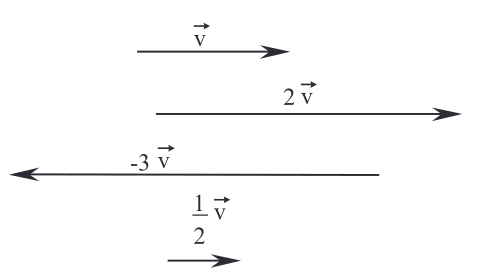
\includegraphics[width=0.5\textwidth]{./fig/fig1.19.png}
    \caption{Multiplicação por escalar}\label{fig:fig1.19}
\end{figure}

Além disso:
\begin{itemize}
    \item Todos os vetores $\alpha \overrightarrow{v}$, para $\alpha \in
      \mathbb{R}$, pertencem a uma mesma reta paralela a $\overrightarrow{v}$.
    \item Se $\overrightarrow{u} \parallel \overrightarrow{v}$ e
      $\overrightarrow{v} \neq \overrightarrow{0}$, então existe $\alpha \in
      \mathbb{R}$ tal que $\overrightarrow{u} = \alpha \overrightarrow{v}$.
    \item A cada vetor $\overrightarrow{v} \neq \overrightarrow{0}$, associamos
      dois vetores unitários paralelos a $\overrightarrow{v}$. O versor de
      $\overrightarrow{v}$ é dado por:
      \begin{align*}
        \overrightarrow{v} &= \frac{\overrightarrow{v}}{|\overrightarrow{v}|} \\
        \text{Exemplo: } |\overrightarrow{v}| &= 5, \text{ o versor de }
        \overrightarrow{v} = \frac{\overrightarrow{v}}{|\overrightarrow{v}|}
      \end{align*}
\end{itemize}

\newpage

\subsection{Exemplos}

\question{
  Representados os vetores \( \overrightarrow{u} \), \( \overrightarrow{v} \) e
  \( \overrightarrow{w} \) como na Figura~\ref{fig:fig1.20}, obter graficamente
  o vetor \( \overrightarrow{w} \) tal que \( \overrightarrow{x} =
  2\overrightarrow{u} − 3\overrightarrow{v} + \frac{1}{2}\overrightarrow{w} \)
}
\begin{figure}[H]
  \centering
  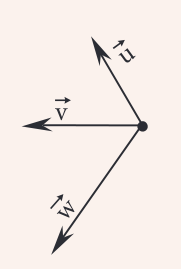
\includegraphics[width=0.3\textwidth]{./fig/fig1.20.png}
  \caption{}\label{fig:fig1.20}
\end{figure}
\answer{
  \begin{figure}[H]
    \centering
    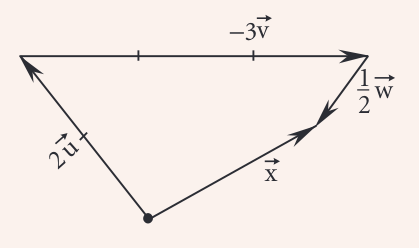
\includegraphics[width=1\textwidth]{./fig/q5.png}
  \end{figure}
}

\newpage

\question{
  Demonstrar que o segmento cujos extremos são os pontos médios de dois lados 
  de um triângulo é paralelo ao terceiro lado e igual à sua metade.
}
\answer{
Seja o triângulo \(ABC\) e \(M\) e \(N\) os pontos médios dos lados \(CA\) e
\(CB\), respectivamente (Figura~\ref{fig:q6}).  Pela figura, tem-se  

\[
  \begin{align*}
    \overrightarrow{MN} &= \overrightarrow{MC} + \overrightarrow{CN} \\
    &= \frac{1}{2} \overrightarrow{AC} + \frac{1}{2} \overrightarrow{CB} \\
    &= \frac{1}{2} \left( \overrightarrow{AC} + \overrightarrow{CB} \right) \\
    &= \frac{1}{2} \overrightarrow{AB} \\
  \end{align*}
\]

Logo, conclui-se que \( \overrightarrow{MN} \parallel \overrightarrow{AB} \) e
\( |\overrightarrow{MN}| = \frac{1}{2} |\overrightarrow{AB}| \).

  \begin{figure}[H]
    \centering
    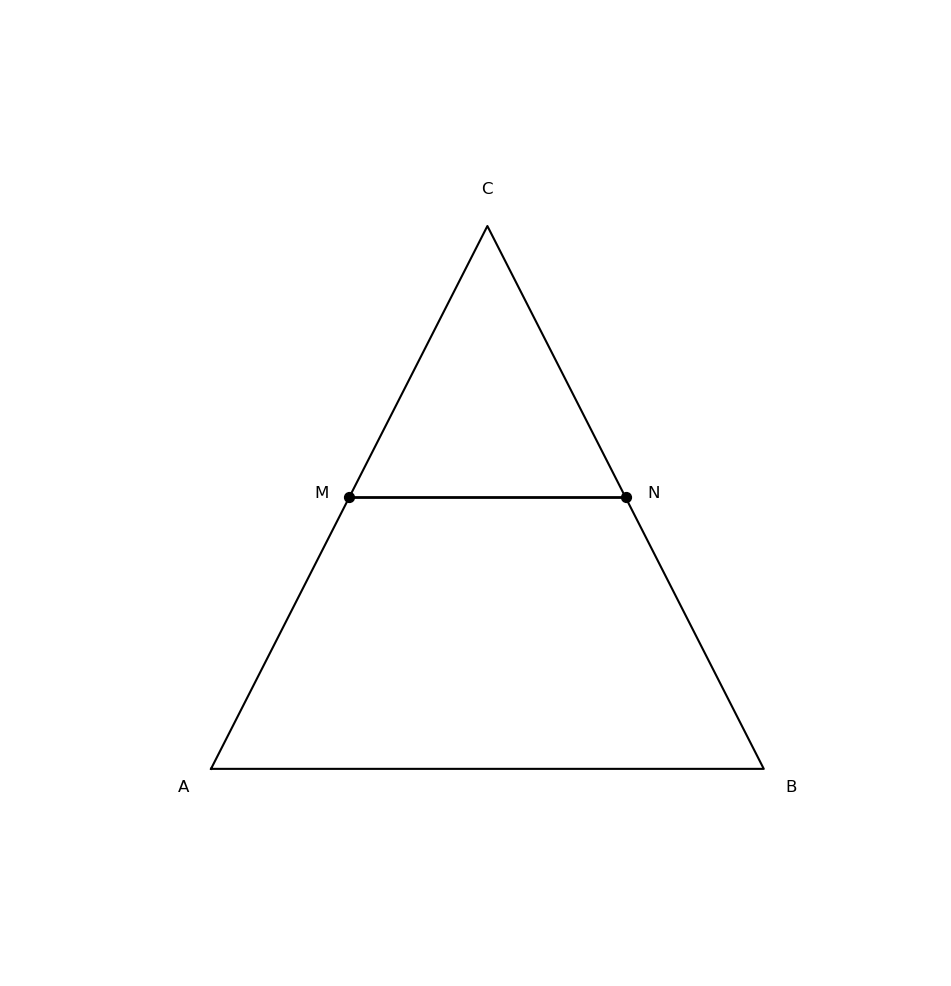
\includegraphics[width=0.9\textwidth]{./fig/q6.png}
    \caption{}\label{fig:q6}
  \end{figure}
}
